\documentclass[12pt]{article}
%\usepackage[utf8]{inputenc}
%\documentclass[UTF8]{ctexart}
%\usepackage[UTF8, heading = false, scheme = plain]{ctex}
\usepackage{geometry}
%geometry{a4paper,scale=0.9}
\geometry{a4paper,left=1cm,right=1cm,top=1cm,bottom=2cm}
\usepackage{amsfonts}
\usepackage{color}
\usepackage{url}
%\usepackage{biblatex}
\usepackage{amsmath}
\usepackage{amssymb}
\usepackage{latexsym}
\usepackage{cite}
%\addbibresource{ref.bib}
%\bibliography{ref.bib}
\usepackage{caption}
\usepackage{graphicx, subfig}
\usepackage{float}
%\usepackage[fontset=ubuntu]{ctex}
%\usepackage{fontspec}
\usepackage{xeCJK}
%\usepackage[colorlinks,
%anchorcolor=black,
%citecolor=black]{hyperref}
%\setmainfont{SimSun}
\usepackage[section]{placeins}
\usepackage{enumitem}
\usepackage{framed}
\usepackage[framemethod=TikZ]{mdframed}
\usepackage{indentfirst}
\usepackage{setspace}%使用间距宏包
\linespread{1.5}

\title{Uplift Model介绍\cite{Uplift_Model_In_One_Article}\cite{Uplift_Model_In_Ali}}
\author{leolinuxer}
%\date{June 2020}

\begin{document}
%\setlength{\parindent}{0pt}
\maketitle
\tableofcontents

\section{背景介绍}
目前,智能化的营销手段越来越普及,商家可以通过多种渠道触达消费者,比如,在手淘上商家可以圈定他想要的目标人群,进行广告推送,为店铺拉新,也可以通过短信或旺旺这些渠道定向发放优惠券。无论是红包还是广告,我们都称为营销的干预手段,其背后都是有成本的。营销的目标就是在成本有限的情况下最大化营销的总产出,这里面最关键的一点是我们能否准确找到真正能被营销打动的用户,我们称他们为营销敏感人群。

Uplift models用于预测一个treatment的增量反馈价值。举个例子来说,假如我们想知道对一个用户展现一个广告的价值,通常的模型只能告诉我们用户在展示广告后的购买意愿很强,但事实很有可能是他们在被展示广告之前就已经很想购买了。Uplift models聚焦于用户被展示广告后购买意愿的增量。

\section{背景和问题定义}
传统模型通常直接预测目标(用户被 treat 后,行为 buy 的概率):
$$
Outcome = P(buy \  | \ treatment)
$$


\textbf{Uplift models预测增量值,也就是lift的部分}(用户是否被treat,行为 buy 的概率差):
$$
Lift = P(buy \  | \ treatment) - P(buy \ | \ no \ treatment)
$$

这里我们用用户买不买来举个例子(但这里的目标可以根据具体场景改变)。个体在面对treated或者untreated之后的反应可以分为下面四种:
\begin{figure}[H]
    \centering
    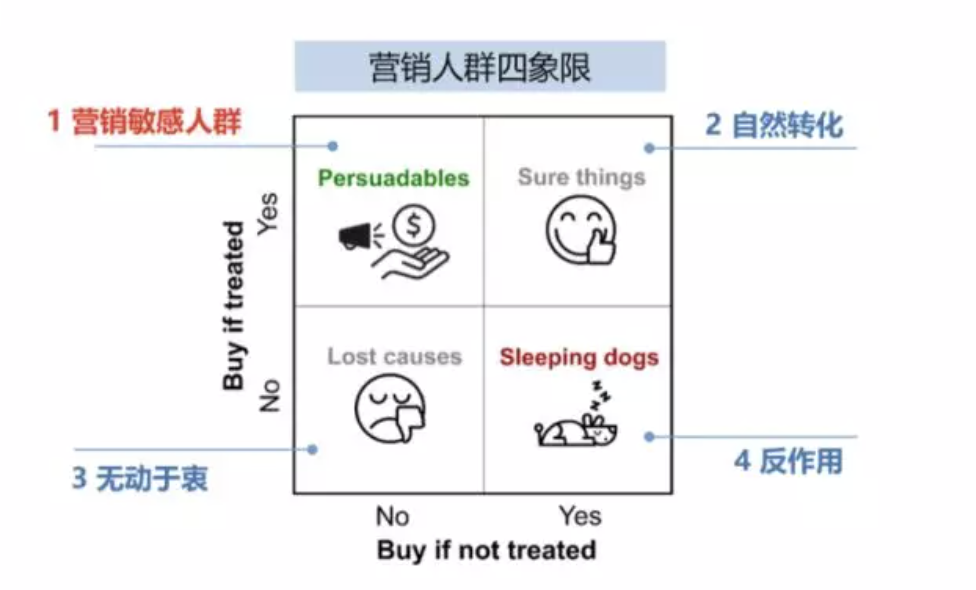
\includegraphics[width=.8\textwidth]{fig/CasualInference-Uplift-Model-Population.png}
\end{figure}

图表解读:
\begin{itemize}
\setlength{\itemsep}{0pt}
\setlength{\parsep}{0pt}
\setlength{\parskip}{0pt}
    \item 横坐标:左边-用户不被treat,不会购买;右边-用户不被treat,会购买;
    \item 纵坐标:上边-用户被treat,会购买;下边-用户被treat,不会购买;
    \item 所以有四象限的人群:
    \begin{itemize}
\setlength{\itemsep}{0pt}
\setlength{\parsep}{0pt}
\setlength{\parskip}{0pt}
    \item 左上:不treat时,不购买,treat 后,购买(营销敏感人群)
    \item 右上:不treat时,购买,treat 后,购买(自然转化)
    \item 左下:不treat时,不购买;treat 后,不购买(无动于衷)
    \item 右下:不treat时,购买;treat 后,不购买(反作用)
\end{itemize}
\end{itemize}

比如,我们对人群做四象限的划分,横纵坐标分别是用户在有干预和无干预情况下的购买状况。如上图,左上角人群的购买状况在干预后发生了正向变化,如果我们不对这类人群进行干预,那他有可能是不购买的,但是干预之后的购买概率有极大提升,所以这类人群是我们真正想要触达的用户,即\textbf{营销敏感人群}。而其他人群比如第2类和第3类,在干预前后的购买状况没有变化,所以预算花费可能是浪费。右下角是一类比较特殊的人群,虽然其在干预前后的状态有跳变,但这种跳变不是我们希望看到的,因为确实有一些人群对营销是反感的,所以对这类人群我们应该极力避免触达。Uplift Model正是为了识别我们想要的营销敏感人群。

但是在现实生活中我们却没有办法准确的判断一个人是属于哪种类型,因为我们不可能对同一个用户同时treat和no treat。但是借助统计和机器学习的知识,我们就可以得到\textbf{相似的用户大致会怎么反应}。这就是uplift模型的核心,每一个用户会得到一个位于-1到1的lift score,用于指导用户人群的选择。

因此整个问题可以表述为:
\begin{figure}[H]
    \centering
    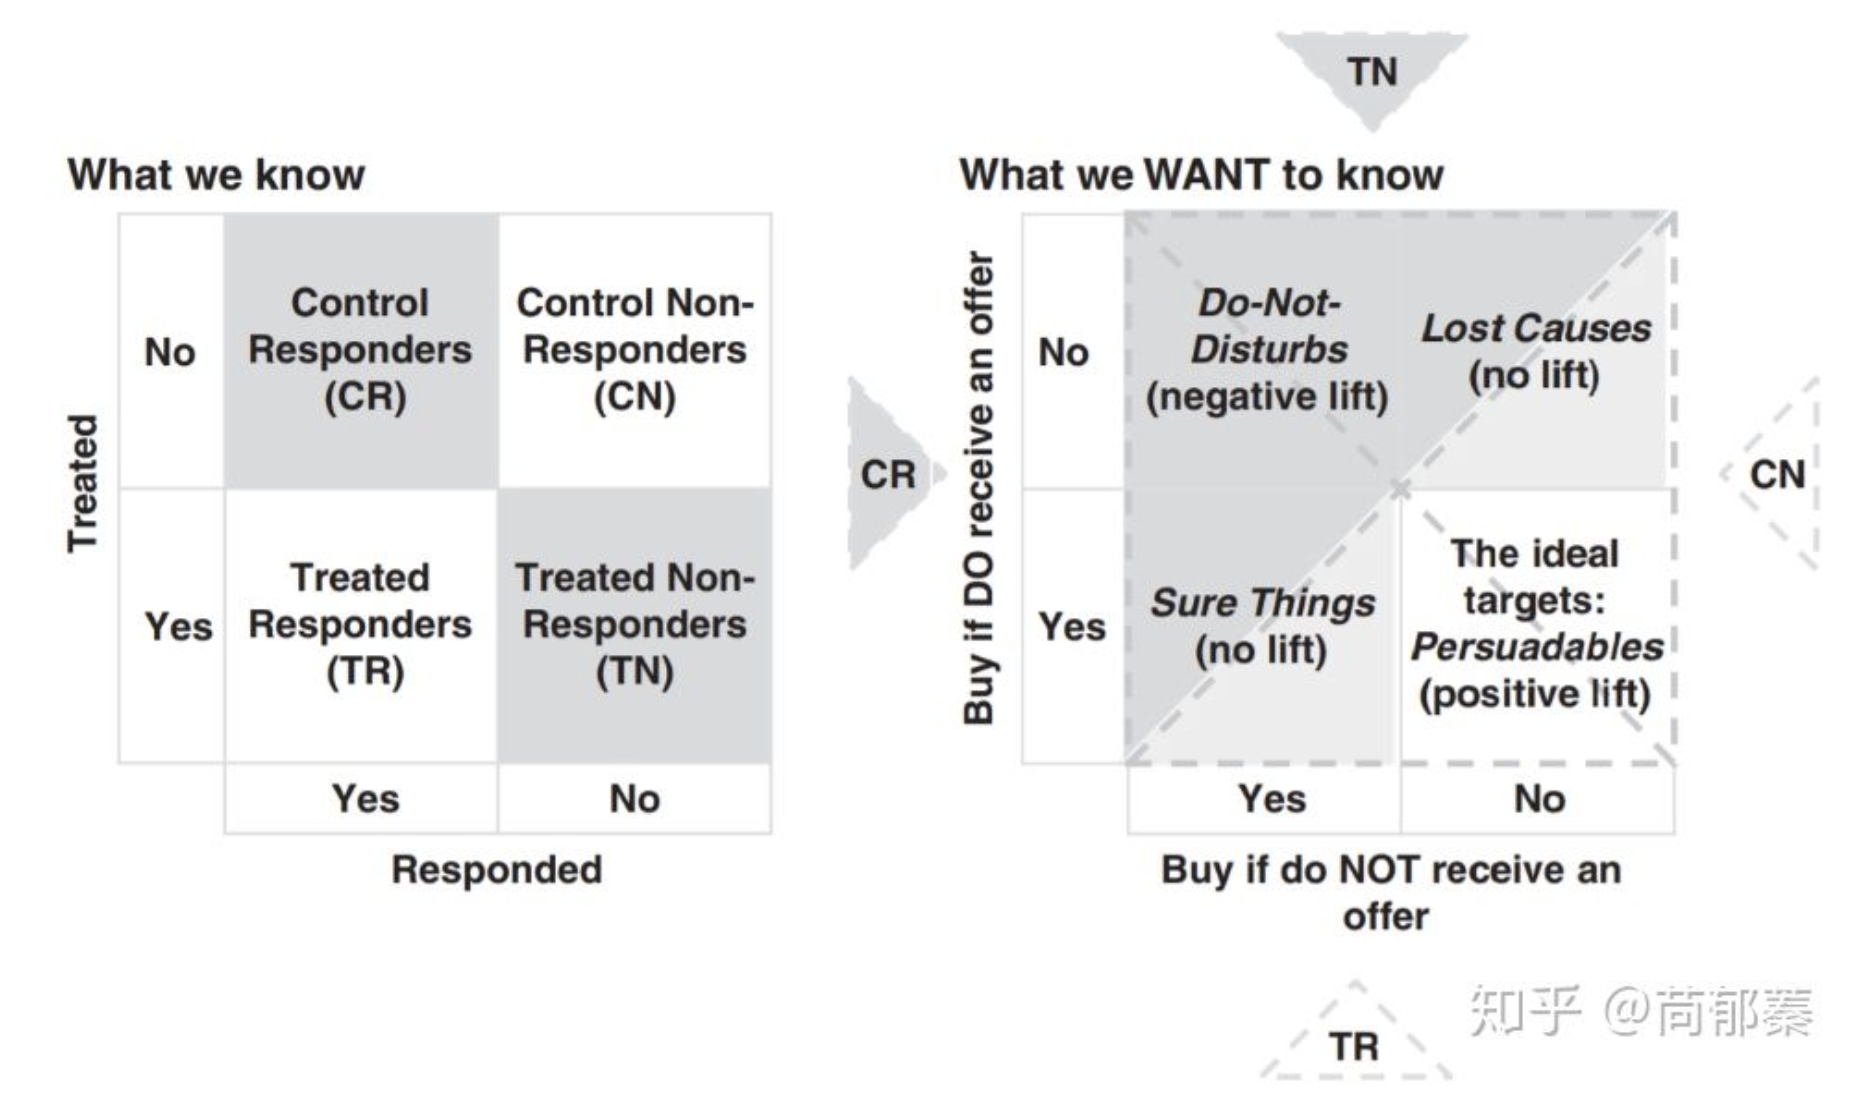
\includegraphics[width=1\textwidth]{fig/CasualInference-Uplift-Model-Problem.png}
\end{figure}

我们能获得的数据,是不同用户在treat或者no treat 下的 response(responder 或 non-responder);我们希望挖掘出来的是,用户如果不treat,是否buy;如果 treat,是否buy;

\section{Uplift Model的价值}
接下来介绍什么是Uplift Model,以及Uplift Model和传统的Response Model有什么样的差异。以广告投放为例,对于两个用户群,我们知道他们对广告投放的转化率分别是0.8\%和2\%,假如只有一次广告曝光的机会,应该向哪类用户投放广告?

按照以往的经验和直觉,可能会向第二类用户群投放广告,因为其转换率是最高的,但这个结论是对的吗?经过进一步分析,除了广告曝光转化率之外,,我们还能知道这两类用户群体在没有广告触达情况下的自然转化率(比如分别是:0.2\%和1.7\%),从而推算出广告所带来的增量。

比如第一类用户的广告转化率虽然低,但在没有广告触达情况下的转化率更低,即广告所带来的增量(uplift = 0.8\% - 0.2\% = 0.6\%)反而是比第二个用户更高的(uplift = 2\% - 1.7\% = 0.3\%),而我们要最大化总体的转化率其实等价于最大化广告的增量,按照这个逻辑,我们应该向第一个用户投放广告。也就是说Response Model很有可能会误导我们做出错误的决策,Uplift Model和Response Model之所以有差异,主要在于两个模型的预测目标不一样:
\begin{itemize}
\setlength{\itemsep}{0pt}
\setlength{\parsep}{0pt}
\setlength{\parskip}{0pt}
    \item Response Model:\textbf{看过}广告之后购买的概率,这本身是一个相关性(correlation,无法区分营销敏感人群和自然转化人群)
    \item Uplift Model:\textbf{因为}广告而购买的概率,这是一个因果推断的问题(causation,精准定位营销敏感人群)
\end{itemize}

\section{建模方法}
\subsection{形式化的定义}
$$
p(Y_i|X_i, T_i = 1) - p(Y_i|X_i, T_i = 0) 
$$
其中,$Y$为Potential Outcome,$X$为User Feature, $T$为Treatment indicator;

也就是说,$Y$代表结果 ( 比如用户的点击,转化等 ),$X$是用户维度的特征,$T$代表的是营销的变量 ( 1代表有干预,0代表无干预 )。

因此这个概率差值表示的是用户在有干预和没有干预情况下的变化,这个模型建模的难点在于我们获取到的训练数据是不完整的,对于个体来说,我们不可能同时观测到在有干预和没有干预两种情况下的表现,也就是因果推断中经常提到的\textbf{反事实}的问题。

\begin{framed}
进一步理解\cite{Uplift_Model_Principle_And_Practice}:

假设有 $N$ 个用户,$Y_i(1)$ 表示我们对用户$i$干预后的结果,比如给用户 $i$ 发放优惠券后(干预)用户下单(结果),$Y_i(0)$ 表示没有对用户干预的情况下用户的输出结果,比如没有给用户 $i$ 发放优惠券(干预),用户下单(结果)。用户 $i$ 的因果效应(causal effect)的计算方式就是:
$$
\tau_i = Y_i(1) - Y_i(0) \qquad \qquad (1) 
$$

\textbf{Uplift Model 的目标就是最大化$\tau_i$}。这是一个增量,即有干预策略相对于无干预策略的提升,简单讲就是干预前后结果的差值。

实际使用时会取所有用户的因果效应期望的估计值来衡量整个用户群的效果,称为\textbf{条件平均因果效应(Conditional Average Treatment Effect, CATE)}:
$$
CATE: \tau(X_i) = E[Y_i(1)|X_i] - E[Y_i(0)|X_i] \qquad \qquad (2)
$$

上式中 $X_i$ 是用户 $i$ 的特征,所谓的 conditional 指基于用户特征。

(2)式是理想的uplift计算形式,实际上,对用户$i$我们不可能同时观察到使用策略(treatment)和未使用策略(control)的输出结果,即不可能同时得到$Y_i(1)$和$Y_i(0)$。因为对某个用户,我们要么发优惠券,要么不发。将(2)式修改一下:
$$
Y_i^{obj} = W_iY_i(1) + (1-W_i)Y_i(0)
$$

其中$Y_i^{obs}​$是用户 $i$ 可以观察到的输出结果,$W_i$ 是一个二值变量,如果对用户 $i$ 使用了策略,$W_i = 1$,否则$W_i = 0$。

在条件独立的假设下,条件平均因果效应的期望估计值是:
$$
\tau(X_i) = E[Y_i^{obj}|X_i = x, W = 1] - E[Y_i^{obj}|X_i = x, W = 0] 
$$

上式要满足条件独立(CIA)的条件,即用户特征与干预策略是相互独立的:
$$
\{Y_i(1), Y_i(0)\} \bot W_i|X_i
$$

实践上,\textbf{满足CIA这样条件的样本的可以通过AB实验获取},因为时随机实验,可以保证用户(特征)与干预策略是相互独立的。

增益模型要优化 $\tau(X_i)$,值越高越好。然而一个用户不能同时观察到使用干预策略和不使用干预策略的结果,因此 $\tau(X_i)$ 是难以直接优化的。但如果通过AB实验,可以获得使用干预策略和不使用干预策略两组人群。因为通过A/B Test拆分流量得到的这两组样本在特征的分布上面是一致的。如果两组人群的特征分布一致,可以通过模拟两组人群的 $\tau(X_i)$ 得到个体用户的 $\tau(X_i)$。因此增益模型依赖AB实验的数据,\textbf{随机化实验是Uplift Model建模过程中非常重要的基础设施}。
\end{framed}

我们应当如何去建模呢?可以从人群的角度来对平均因果效应做统计,假设我们有两群\textbf{同质}用户,均来自一线城市/年龄段为25-35/女性,我们可以对其中一组用户进行广告投放,另外一组不进行任何干预,之后统计这两群人在转化率上的差值,这个差值可以被近似认为是具备同样特征的人可能的平均因果效应。所以Uplift Model本质是从训练样本中学习条件的平均因果效应,同时因为模型是具有一定的泛化能力,可以对没有见过的样本也进行预测。


\subsection{The transformed outcome tree}
Uplift models需要每一个人的两方面信息:是否给予treatment,产出label。理想情况下,我们可以得到一些个体在随机分配到实验组(treat group)和对照组(control group)后的数据,基于他们对于treatment的反应,outcome label可以被转化为下面这个矩阵(Athey and Imbens 2016)(实际情况中可以有其他的正负样本划分方法):
\begin{figure}[H]
    \centering
    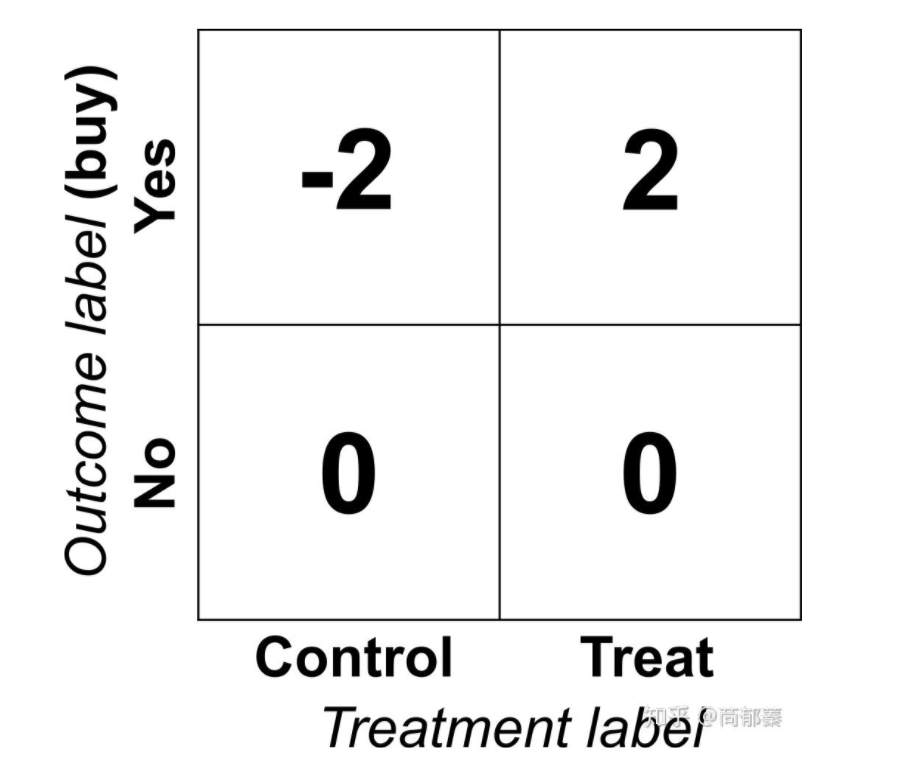
\includegraphics[width=.5\textwidth]{fig/CasualInference-Uplift-Model-Label.png}
\end{figure}

可能在第一眼的时候觉得这个目标矩阵不太靠谱,像拍脑袋的结果,为啥没有买的给不给treatment都是0?为什么给了treatment买了就是2?看起来非常不直观,但是是有道理在里面的,假如将一群人随机分为控制组和对照组,最后得到的平均值矩阵就是这群人的lift。

为了说明这个问题,考虑有一群人,人数为$2n$,其中$n$个给了treatment $t$,另外$n$个不给作为对照组。为了简单起见我们将$i =1 ,…, n$为treatment组$t$,$i =n+1 ,…, 2n$为控制对照组$c$。对于每一个用户,原始的outcomes和转换后的分别为 $y_i$ 和 $z_i$,那么对于这群人,对于购买行为的lift为:

\begin{align*}
Lift & = E[y|t] - E[y|c] \\
      & = \frac{1}{n}\sum_{i=1}^ny_i - \frac{1}{n}\sum_{i=n+1}^{2n}y_i \\
      & = \frac{1}{2n}[\sum_{i=1}^n2y_i - \sum_{i=n+1}^{2n}2y_i]  \\
      & = \frac{1}{2n}\sum_{i=1}^{2n}z_i \\
      & = E[z]
\end{align*}

也就是说,转化后的outcome取决于前一个group的lift,这个优雅的转换大大简化了lift问题,我们可以直接对$z$建立回归模型,我们就可以得到对于基于特征x表征的用户的uplift:
$$
\text{uplift}(x) = E[y|x,t] - E[y|x,c] = E[z|x]
$$


\subsection{建模方法}
\subsubsection{Two-Model(差分响应模型)}
最简单的Uplift建模方法是基于Two Model的差分响应模型,它的形式和前面介绍的Uplift Model的定义非常相似,包含了两个响应模型,其中\textbf{一个模型$G$用来估计用户在有干预情况下的响应},另外\textbf{一个模型$G'$是用来学习用户在没有干预情况下的响应}。也就是说,预测时时分别对实验组模型和对照组模型预测用户的分数,两个模型预测分数相减就得到了uplift score之后将两个模型的输出做差,就得到我们想要的uplift。

简单来说,就是训练2个模型,首先圈定一个人群(同质人群),里面有被投放广告的,也有没有投放广告的,注意两个人群(投放广告与没有投放广告)的选取一定要有随机性。其中未投放广告的为对照组,投放广告的为实验组。对两个人群分别建模,分别为model1和model2,当新来一个该圈定的同质人群流量,会分别输入到moedl1和model2分别得到p1和p2,p2-p1就是该用户流量的增益\cite{Understand_Uplift_Model_In_Ads}。

这种建模方法的优点是比较简单容易理解,同时它可以套用我们常见的机器学习模型,如LR,GBDT,NN等,所以该模型的落地成本是比较低的,但是该模型最大的缺点是精度有限,这一方面是因为我们独立的构建了两个模型,这两个模型在打分上面的误差容易产生累积效应,第二是我们建模的目标其实是response而不是uplift,因此对uplift的识别能力比较有限。

\begin{figure}[H]
    \centering
    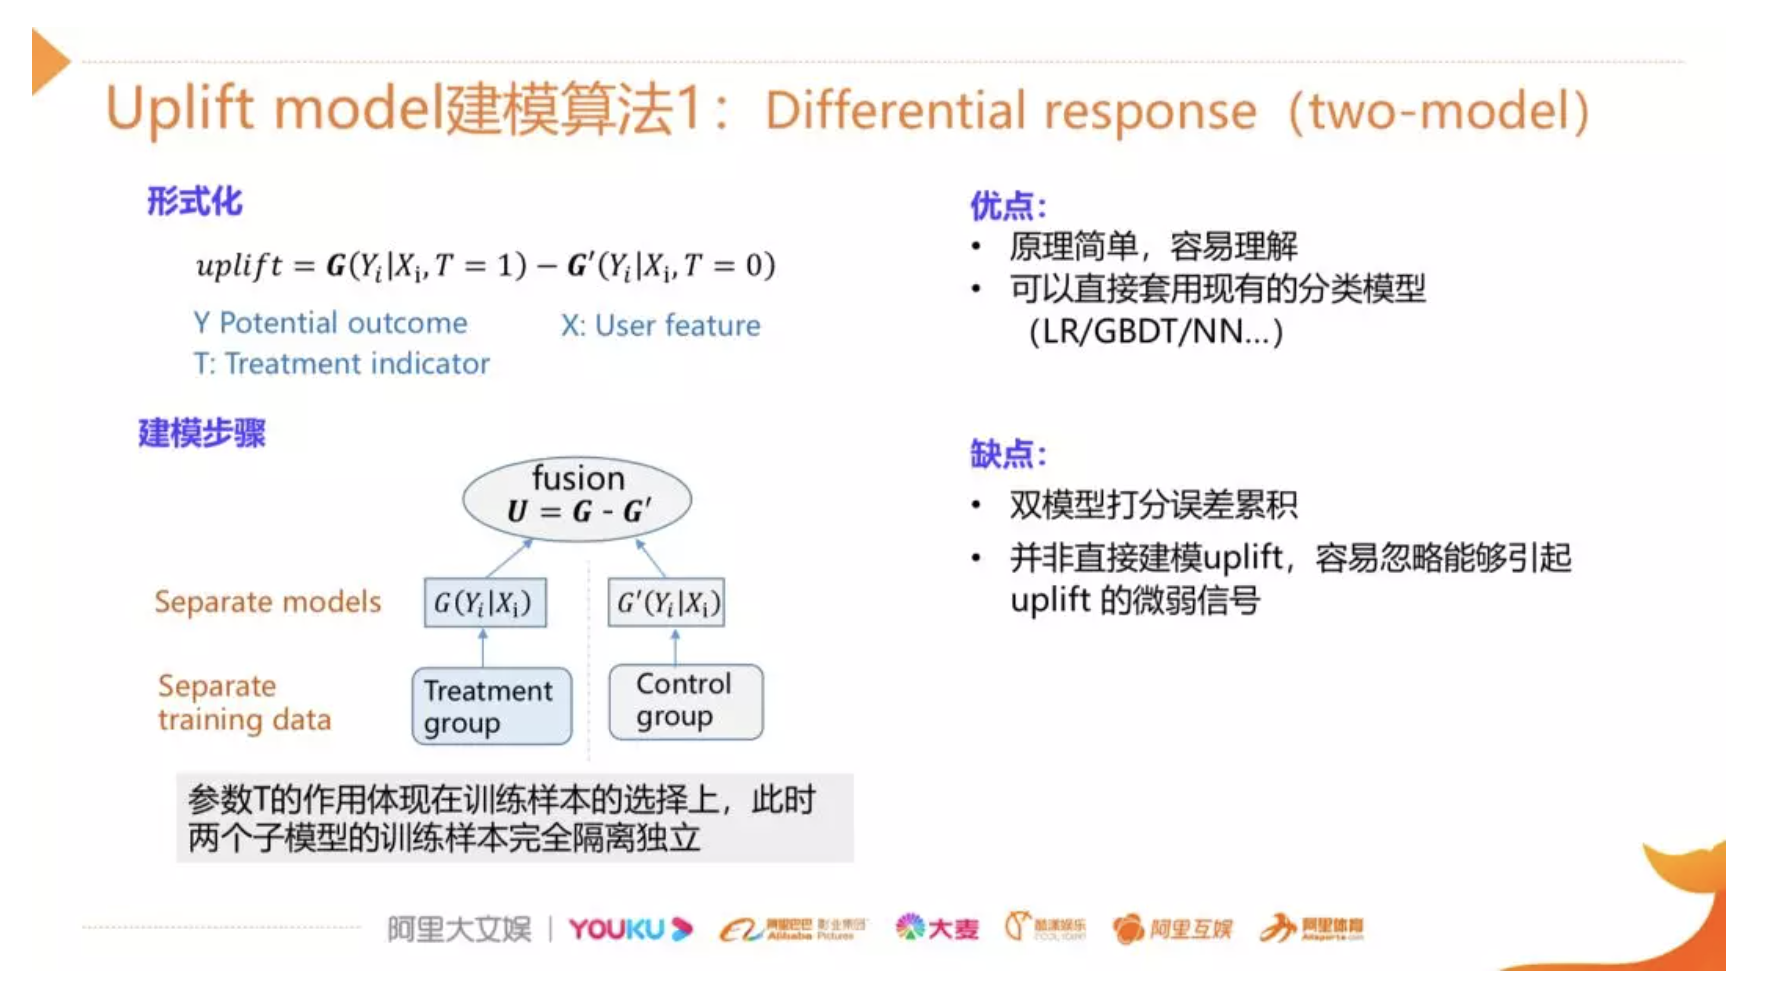
\includegraphics[width=1\textwidth]{fig/CasualInference-Uplift-Model-Two-Model.png}
\end{figure}

\begin{framed}
公式表述\cite{Uplift_Model_Principle_And_Practice}:

实验组是使用干预策略的用户(treatment),对照组是未使用干预策略的用户(control),正样本都是下单用户。即分别使用两个模型优化$E[Y_i^T|X_i^T]$和$E[Y_i^C|X_i^C]$,,得到两个模型,分别为:$G_T$和$G_C$。其中,$Y_i^T$和$X_i^T$分别是实验组用户 $i$ 的输出结果和特征;$Y_i^C$和$X_i^C$分别是控制组用户 $i$ 的输出结果和特征。

分别训练好两个模型之后,计算$E[Y^T|X^T] - E[Y^C|X^C]$就得到了条件平均因果效应分数。\textbf{这里因果效应分数是计算出来的而不是通过模型直接优化出来的,所以本质上,这还是传统的响应模型}。

以优惠券发放为例,目标是用户是否下单。训练时取实验组的用户训练,正样本是下单用户,负样本是未下单用户,预测结果是每个用户下单的概率。类似地,对照组也可以使用另一个模型预测出每个用户下单的概率。两个组的用户下单概率求平均,即可得到 $E[Y^T|X^T]$ 和 $E[Y^C|X^C]$,两者相减即得到 $\tau(X)$

预测时,对用户分别使用 $G_T$ 和 $G_C$ 预测,两个模型预测的分数相减即得到预测用户 $i$ 的 $\tau(X_i)$,最后根据 $\tau(X_i)$ 的高低决定是否发券。

\begin{figure}[H]
    \centering
    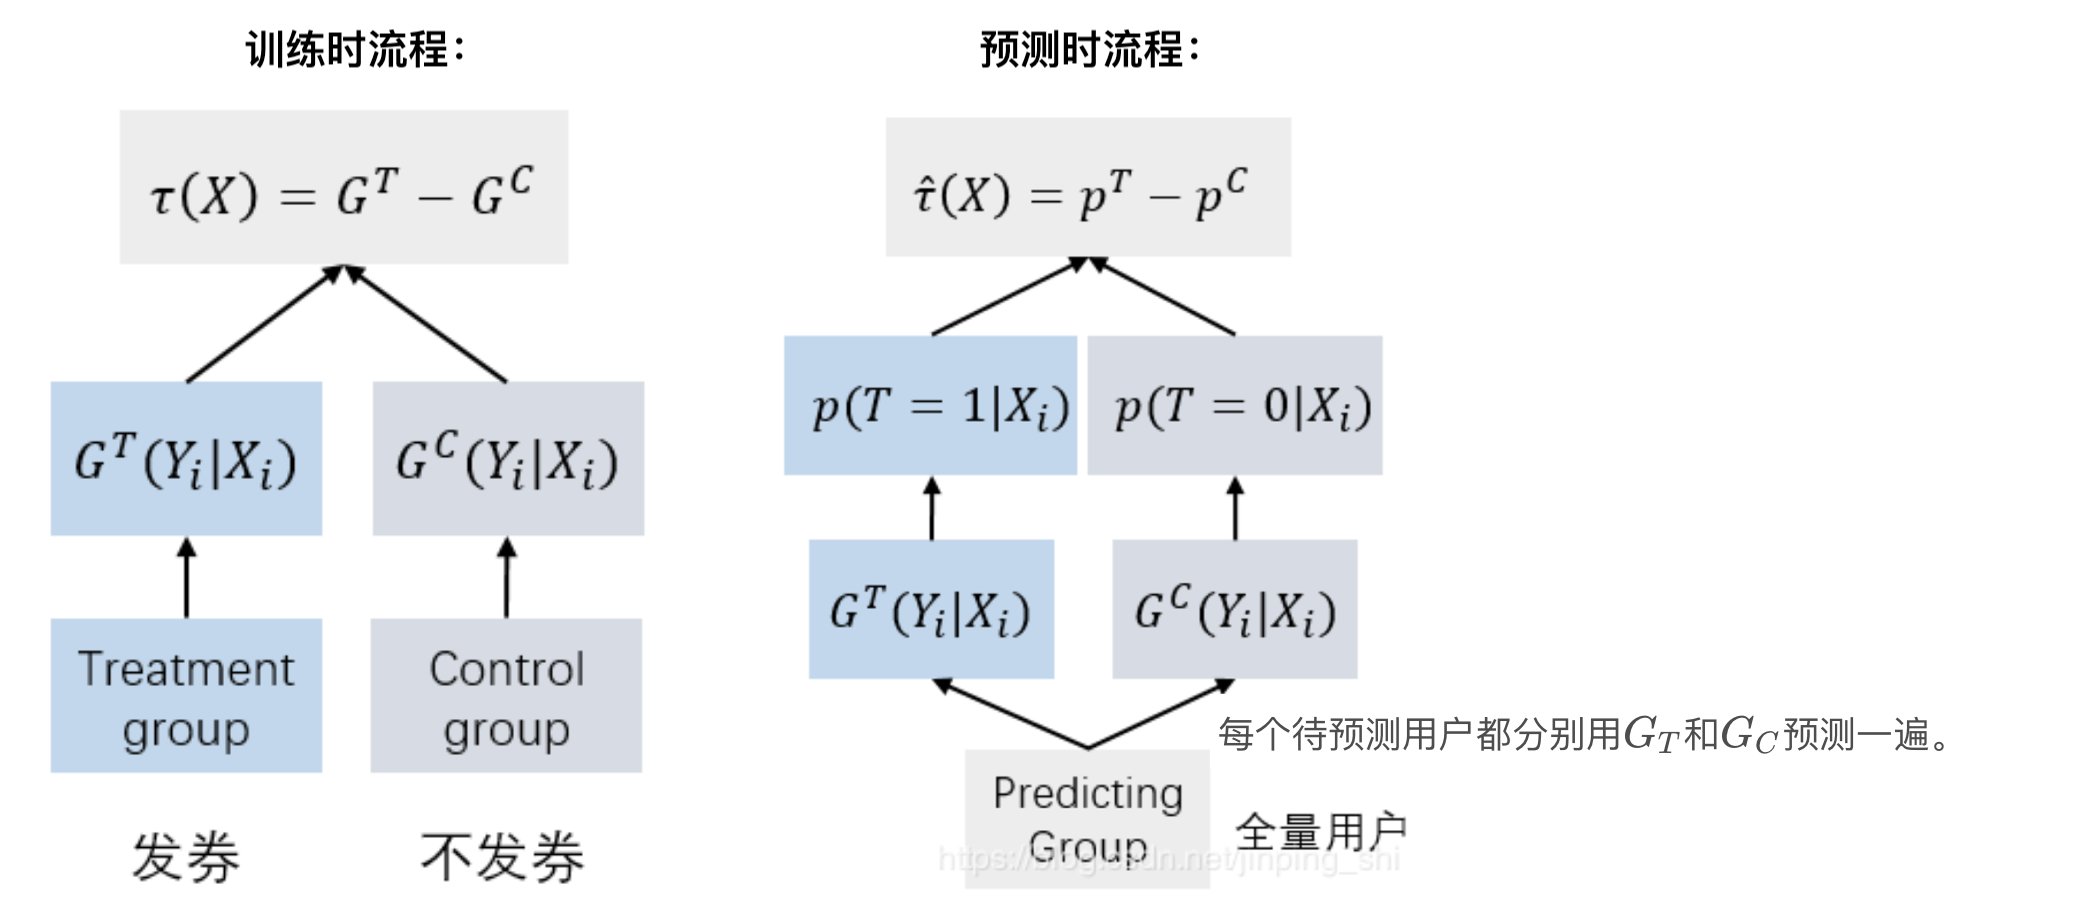
\includegraphics[width=1\textwidth]{fig/CasualInference-Two-Model-Train-Predict.png}
\end{figure}
\end{framed}

Two-Model 模型的优缺点:

差分响应模型简单粗暴,还很直觉。但只是模拟了 $\tau(X_i)$,没有真正优化 $\tau(X_i)$。两个独立的模型分开训练容易累积误差(两个独立模型的误差会累加传递到最终的 uplift score)。不过考虑到实现简单迅速,实践中可以作为baseline使用。

\subsubsection{One-Model(差分响应模型升级版)}
进一步地,还有一个基于One Model的差分响应模型,它和上一个模型最大差别点在于,它在模型层面做了打通,同时底层的样本也是共享的,之所以能实现这种模型层面的打通,是因为我们在样本的维度上做了一个扩展,除了user feature之外,还引入了与treatment相关的变量T ( T如果是0,1的取值可以建模single treatment,T也可以扩展为0到N,建模multiple treatment,比如不同红包的面额,或者不同广告的素材 ),One Model版本和Two Model版本相比最大的优点是训练样本的共享可以使模型学习的更加充分,同时通过模型的学习也可以有效的避免双模型打分误差累积的问题,另外一个优点是从模型的层面可以支持multiple treatment的建模,具有比较强的实用性。同时和Two Model版本类似,它的缺点依然是其在本质上还是在对response建模,因此对uplift的建模还是比较间接,有一定提升的空间,另外,这样是否还能够满足用户特征样与条件策略独立的假设是存疑的。

简单来说,同样首先圈定一个人群(同质人群),里面有被投放广告的,也有没有投放广告的,注意两个人群(投放广告与没有投放广告)的选取一定要有随机性。其中未投放广告的为对照组,投放广告的为实验组,\textbf{把是否被广告干预当作一个特征输入到模型中},然后与用户信息以及上下文信息一起训练一个模型model,当新来一个该圈定的同质人群流量,会分别赋予该流量是否被广告干预特征T=0和T=1,和该广告流量对应的用户信息以及上下文信息一起输入到model中,得到p1和p2,p2-p1就是该用户流量的增益。\cite{Understand_Uplift_Model_In_Ads}。

这里最重要的一点是,干预当成了了一个特征,这样会带来另外一个便利,T可以等于2,3,...(虽然都是广告投放,但是可以是不同的广告投放手段),那么就会给模型的创建带来更大的便利以解决更多的实际场景。

\begin{figure}[H]
    \centering
    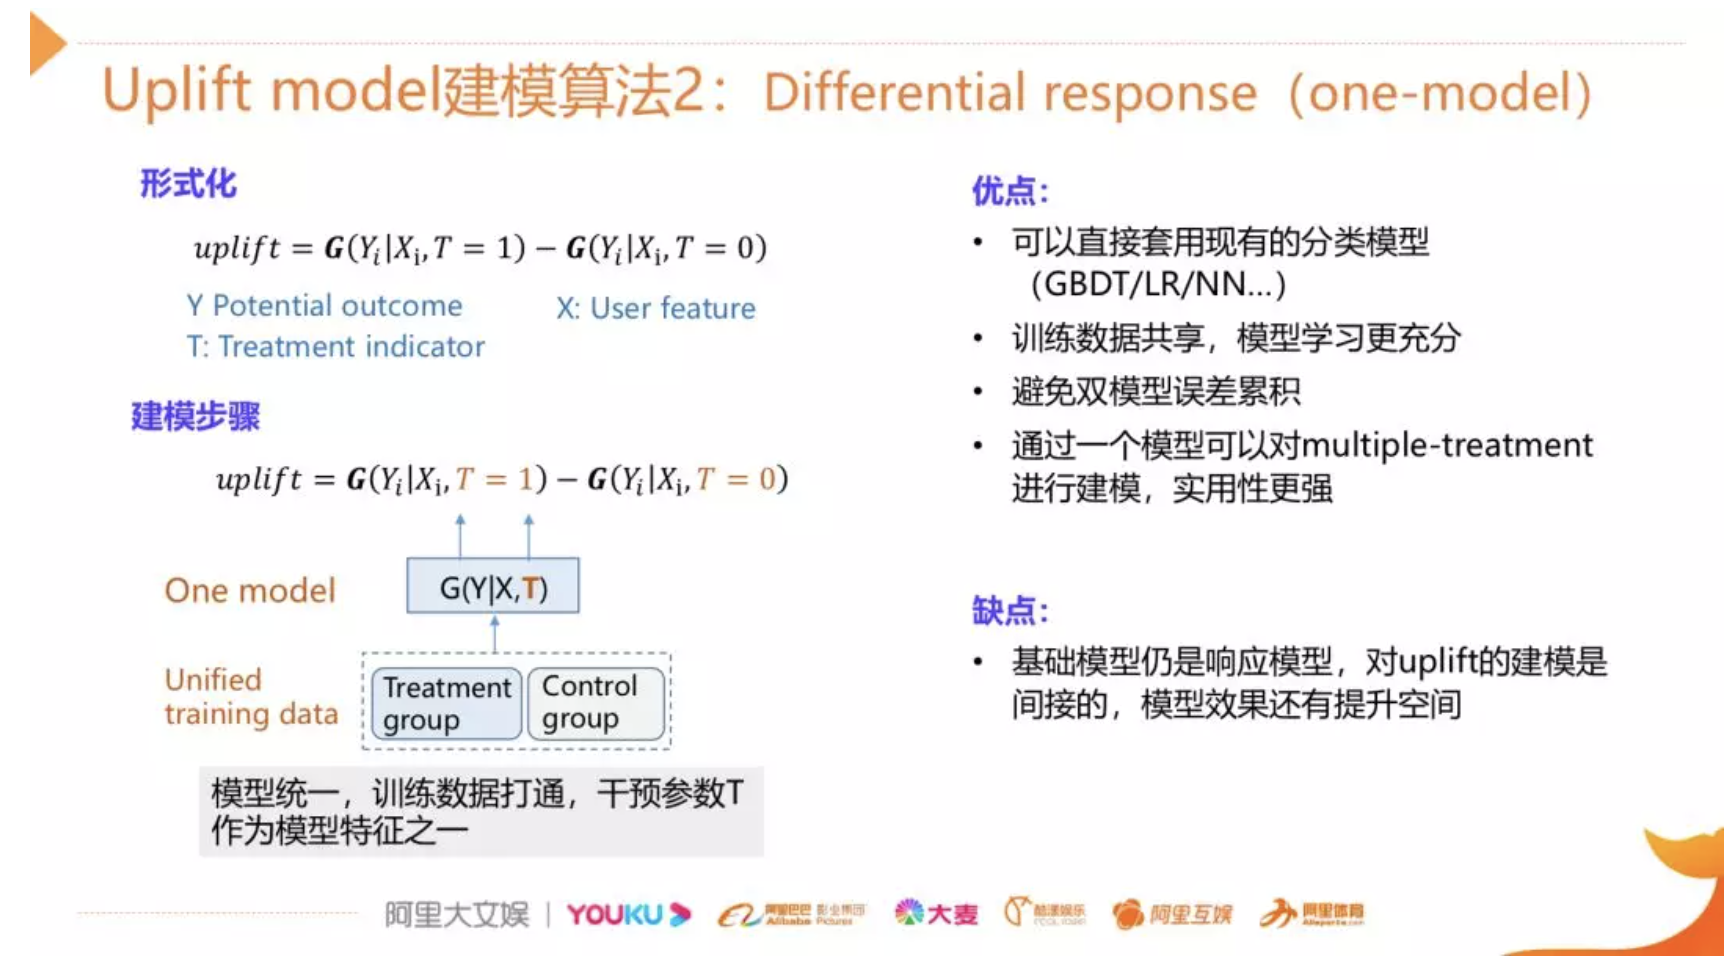
\includegraphics[width=1\textwidth]{fig/CasualInference-Uplift-Model-One-Model.png}
\end{figure}

\subsubsection{Class Transformation Method}
还有一种可以实现实验组对照组数据打通和模型打通的方法叫做class transformation method,可以直接优化 $\tau(X_i)$。

定义一个变量 $G = \{T, C\}$,$G = T$表示有干预,即实验组(treatment),$G = C$表示无干预,即对照组(control);uplift分数 $\tau$ 可以表示为:

\begin{align*}
\tau(X) &= P(Y = 1|X, G = T) - P(Y = 1|X, G = C) \\
	    &= P^T(Y = 1|X) - P^C(Y = 1|X) \qquad \qquad (5)
\end{align*}

上式中 $X$ 表示用户特征,$P^T$ \textbf{表示用户在实验组中下单的概率}(输出结果为positive),$P^C$ \textbf{表示用户在对照组中下单的概率}(输出结果也为positive),uplift score 就是两个概率的差值。

为了统一表示实验组和对照组都下单的情况($Y = 1$),再定义一个变量$Z, Z \in \{0, 1\}$:
$$
Z = \begin{cases}
1 \qquad \text{if} \ G = T \ \text{and} Y = 1 \\
1 \qquad \text{if} \ G = C \ \text{and} Y = 0 \\
0 \qquad \text{otherwise}
\end{cases}
$$

下面证明优化(5)式相当于优化$P (Z=1 | X)$。

假设干预策略 $G$ 与用户相互独立,即 $G$ 独立于 $X$:$P(G|X) = P(G)$,(5)式可以转写为:
\begin{align*}
P(Z = 1|X) &= P(Z=1|X, G=T) P(G = T|X) + P(Z=1|X, G = C)P(G=C|X) \\
	&= P(Y=1|X, G=T) P(G = T|X) + P(Y=0|X, G = C)P(G=C|X) \\
	&= P^T(Y = 1|X)P(G = T) + P^C(Y=0|X)P(G=C) \qquad \qquad (6)
\end{align*}

注意到 $P(G=T)$ 和 $P(G=C)$ 是可以通过AB实验控制的,在随机化实验中,\textbf{如果实验组和对照组的人数是相等的,那么 $P(G=T)=P(G=C)=1/2$,一个用户被分在实验组(有干预策略)和被分在对照组(无干预策略)的概率是相等的}。 在该假设下,(6)式可以改写为:
\begin{align*}
2P(Z=1|X) &= P^T(Y=1|X) + P^C(Y=0|X) \\
	&= P^T(Y=1|X) + 1 - P^C(Y=1|X) \qquad \qquad (7)
\end{align*}

由(7)式可得:
\begin{align*}
\tau(X) &= P^T(Y=1|X) - P^C(Y=1|X) \\
	&= 2P(Z=1|X) - 1 \qquad \qquad (8)
\end{align*}

(8)式就是要计算的uplift score,此时只有$Z$一个变量,可以直接对$Z=1$建模,相当于优化$P(Z=1|X)$,而不需要分别对实验组 $P^T$ 和对照组 $P^C$ 单独建模。而 $P(Z=1|X)$ 可以通过任何分类模型得到,所以这个方法称为Class Transformation Method。

实际上,$Z=1$就是实验组中下单的用户和对照组中未下单的用户,因此可以直接将实验组和对照组用户合并,使用一个模型建模,实现了数据层面和模型层面的打通。\textbf{预测时,模型预测的结果就是uplift score,这点与差分响应模型不同}。

\begin{figure}[H]
    \centering
    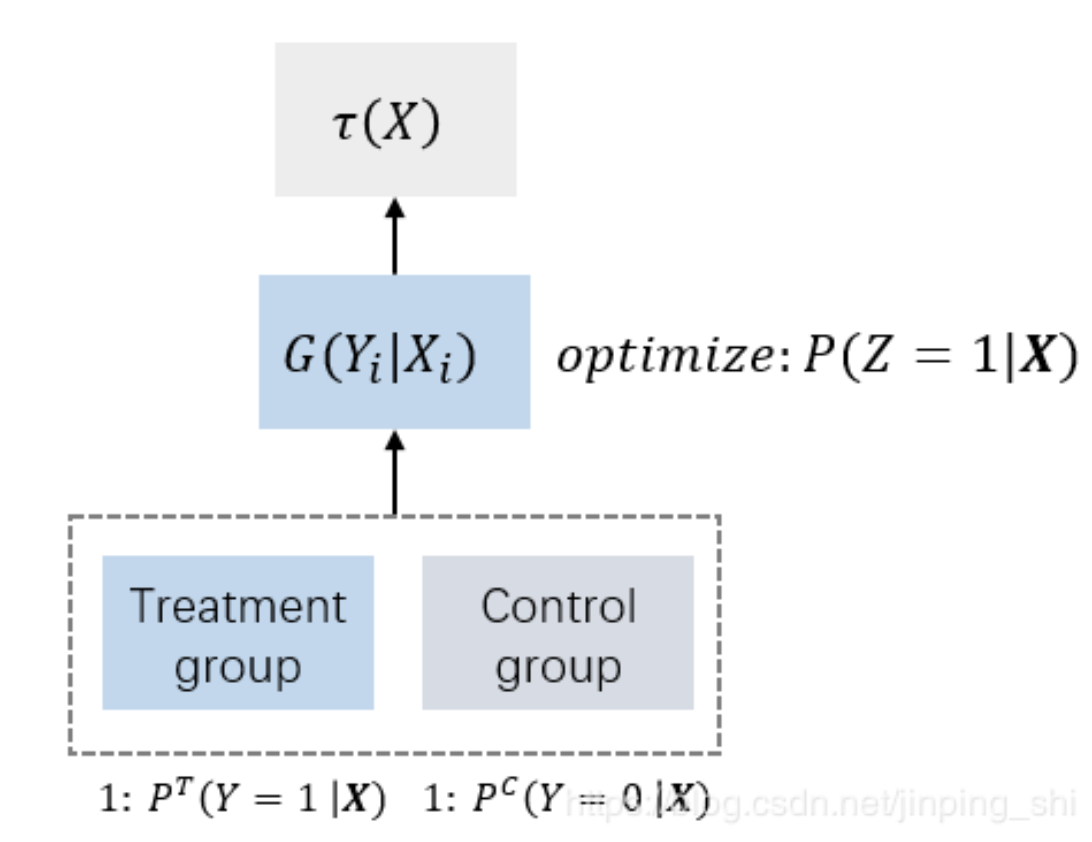
\includegraphics[width=0.6\textwidth]{fig/CasualInference-Uplift-Model-Class-Transformation.png}
\end{figure}

\begin{framed}
\textbf{Class Transformation的两个假设}

该方法有两个假设:
\begin{itemize}
\setlength{\itemsep}{0pt}
\setlength{\parsep}{0pt}
\setlength{\parskip}{0pt}
    \item $G$ 与 $X$ 相互独立;
    \item $P(G=T) = P(G = C) = \frac{1}{2}$
\end{itemize}

第一个假设很好理解,实践中保证用户特征与干预策略无关即可。第二个假设过于严格,难以在实践中每次都满足。但是可以通过\textbf{重采样}使得数据满足该假设,即使不满足(经常会有对照组数量远远小于实验组的情况),根据(6)式,训练数据的不平衡影响的只是 $P(G=T)$ 和 $P(G=C)$ 的权重(原来的权重是1:1),如果模型结果有意义,并且如果在测试集和线上表现良好,那么也不一定非要满足 $P(G=T) = P(G=C) = \frac{1}{2}$ 的假设,实践中都是结果导向。
\end{framed}

\subsubsection{Modeling Uplift Directly}
后续也有相关研究提出了直接的建模方法,通过对现有的模型内部进行深层次的改造来直接刻画uplift,其中研究较多的是基于树模型的uplift建模,下面主要介绍它的思想。

在传统的决策树构建中,最重要的环节是分裂特征的选择,我们常用的指标是信息增益或者信息增益比,其背后的含义还是希望通过特征分裂之后下游节点的正负样本的分布能够更加的悬殊,也就代表类的纯度变得更高。类似的,这种思想也可以引入到Uplift Model的建模过程中,虽然我们并没有用户个体的uplift直接的label,但是我们可以通过treatment组和control组转化率的差异来刻画这个uplift,以图中左下角的图为例,我们有T和C两组样本,绿色的样本代表正样本,红色的代表负样本,可以看到在分裂之前T和C两组正负样本的比例比较接近,但是经过一轮特征分裂之后,T和C组内正负样本的比例发生了较大的变化,左子树中T组全是正样本,C组全是负样本,右子树正好相反,C组的正样本居多,意味着左子树的uplift比右子树的uplift更高,即该特征能够很好的把uplift更高和更低的两群人做一个区分。如何从数学上度量这种概率分布的差异的方式呢?一些文章提出了可行的方法,比如基于KL散度,欧式距离,卡方距离的等等。这种模型的优点是可以直接对uplift进行建模,因此它的精度理论上是更高的,但是在应用层面我们需要做大量的改造和优化,除了前面介绍的分裂规则之外,我们还需要改造它的loss函数,后续的剪枝等一系列的过程,所以它的实现成本是比较高的。

也就是说\cite{Uplift_Model_Principle_And_Practice},该方法\textbf{直接修改树模型的特征分裂计算方法}。常用的特征分裂指标是信息增益(information gain):
$$
\Delta_{gain} = \text{info}_{\text{after}}(D) - \text{info}_{\text{before}}(D)
$$
,可以直接改为:
$$
\Delta_{gain} = D_{\text{after}}(P^T, P^C) - D_{\text{before}}(P^T, P^C)
$$
其中 $D_{\text{before}}(P^T, P^C)$ 和 $D_{\text{after}}(P^T, P^C)$ 分别是分裂前后treatment和control样本的分布,可以用KL散度(KL divergence)、欧氏距离或者卡方距离来刻画这样的分布。

该方法可以直接对uplift建模,理论上精度会很高,但实际应用上除了修改分裂规则外,还需修改loss函数、剪枝算法等,成本较高。

\begin{figure}[H]
    \centering
    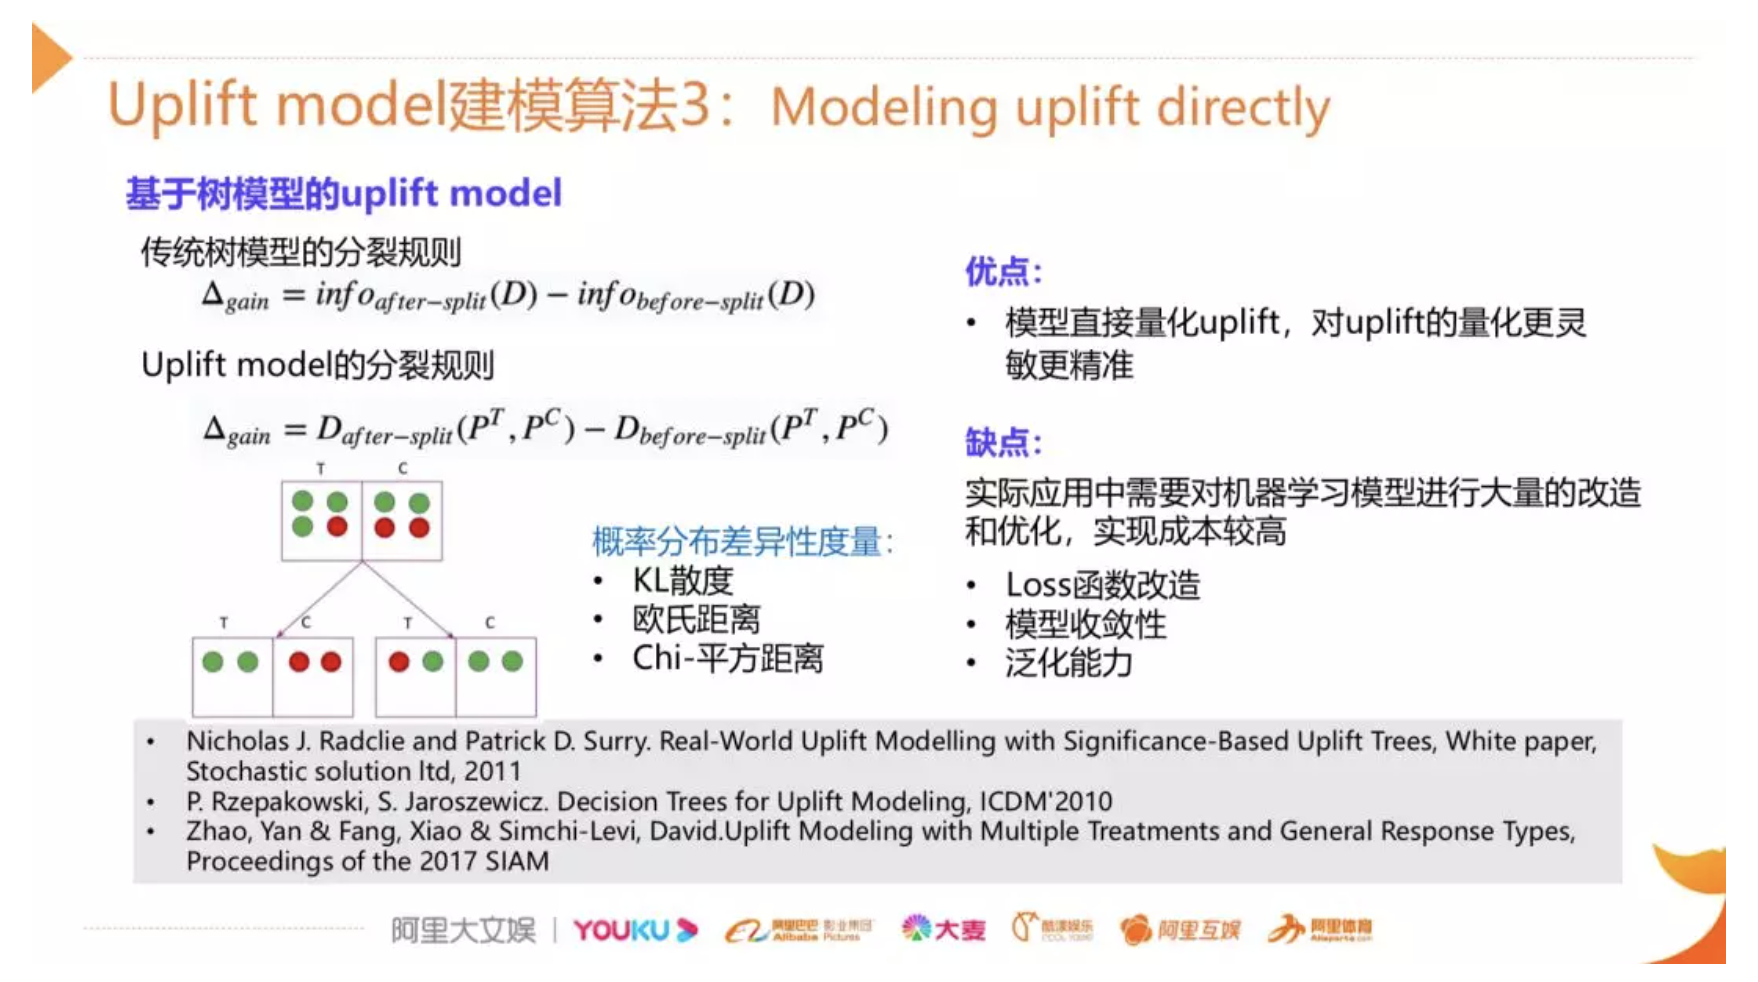
\includegraphics[width=1\textwidth]{fig/CasualInference-Uplift-Model-Direct-Model.png}
\end{figure}

\subsection{Evaluation metrics}
有了以上三种常见uplift的建模方法,我们需要对uplift模型进行评估,因为uplift评估最大的难点在于我们并没有单个用户uplift的ground truth,因此传统的评估指标像AUC是无法直接使用的。

\subsubsection{AUUC曲线}
解决的一个思路是通过构造镜像人群的方式来间接拿到uplift的ground truth,比如说经典的\textbf{AUUC}的指标就是这样去计算的,假设现在有两个满足CIA条件假设的样本组,我们可以对两群人分别预估他们的uplift score,之后将人群按照uplift score进行降序排列,通过score分数这一桥梁,可以把两组人群进行镜像人群的对齐,之后分别截取分数最高的比如10\%的用户出来,计算这一部分人转化率的差异,这个差异就可以近似地认为是分数最高的这群人真实的uplift,类似地,我们可以计算前20\%,40\%一直到100\%的点上面的值,连线就能得到uplift curve。理论上如果模型对uplift的识别比较准确,我们预测uplift比较高的区间段,真实的uplift也较高,uplift curve就会呈现上凸的形式,我们也可以计算曲线下的面积度量不同模型的表现差异。

\subsubsection{Qini指标}
除了上述AUUC曲线,我们下面再介绍一种评估指标,然后介绍如何将这个指标引入Transformed Outcome method。

最典型的评估指标是Qini curve:
$$
Qini = \frac{n_{t,1}(\phi)}{N_t} - \frac{n_{c,1}(\phi)}{N_c}
$$

$n_{t,1}(\phi)$和$n_{c,1}(\phi)$分别代表着对照组和控制组中outcome为1的人数,分数$\phi$表示观察人群占目标人群的比值,$N_t$ 和 $N_c$表示实验组和对照组的总人数(独立于$\phi$),因为$N_t$ 和 $N_c$其实并不独立于$\phi$,也就是实验组和对照组的均衡不是随机的,而是$\phi$的一个函数,所以Qini curve会自然的膨胀。

为了纠正这一点,引入了以下两版曲线:
$$
General \ cumulative \ gains \ curve =  (\frac{n_{t,1}(\phi)}{n_t(\phi)} - \frac{n_{c,1}(\phi)}{n_c(\phi)})\phi
$$

其中$n_t(\phi)$ 和$n_c(\phi)$分别代表了实验组和对照组中观察人群的比例。

首先,我们实现了传统的cumulative gain chart (Gutierrez and Gerardy 2016)。其中$\phi$近似为:
$$
\frac{n_t(\phi) + n_c(\phi)}{N_t + N_c}
$$

这是对uplift的无偏估计。

我们同时也包含了adjusted Qini curve,其中$\phi$ 为:
$$
\frac{n_t(\phi)}{N_t}
$$


\section{Uplift Model在淘票票智能票补中的应用}
下面以淘票票实际场景为例,来说明uplift model如何在实际场景中进行应用。该项目的目标是希望对进入到首页的用户个性化地发送红包,实现在预算和ROI的双重约束下提升平台总体购票转化率。我们的权益就是首页的红包,红包的使用规则、红包类型、预算和交互样式由产品运营设计,算法的作用是实现人和权益的精准匹配,我们需要确定应该给哪些用户发放以及发放哪种类型的权益。
\begin{figure}[H]
    \centering
    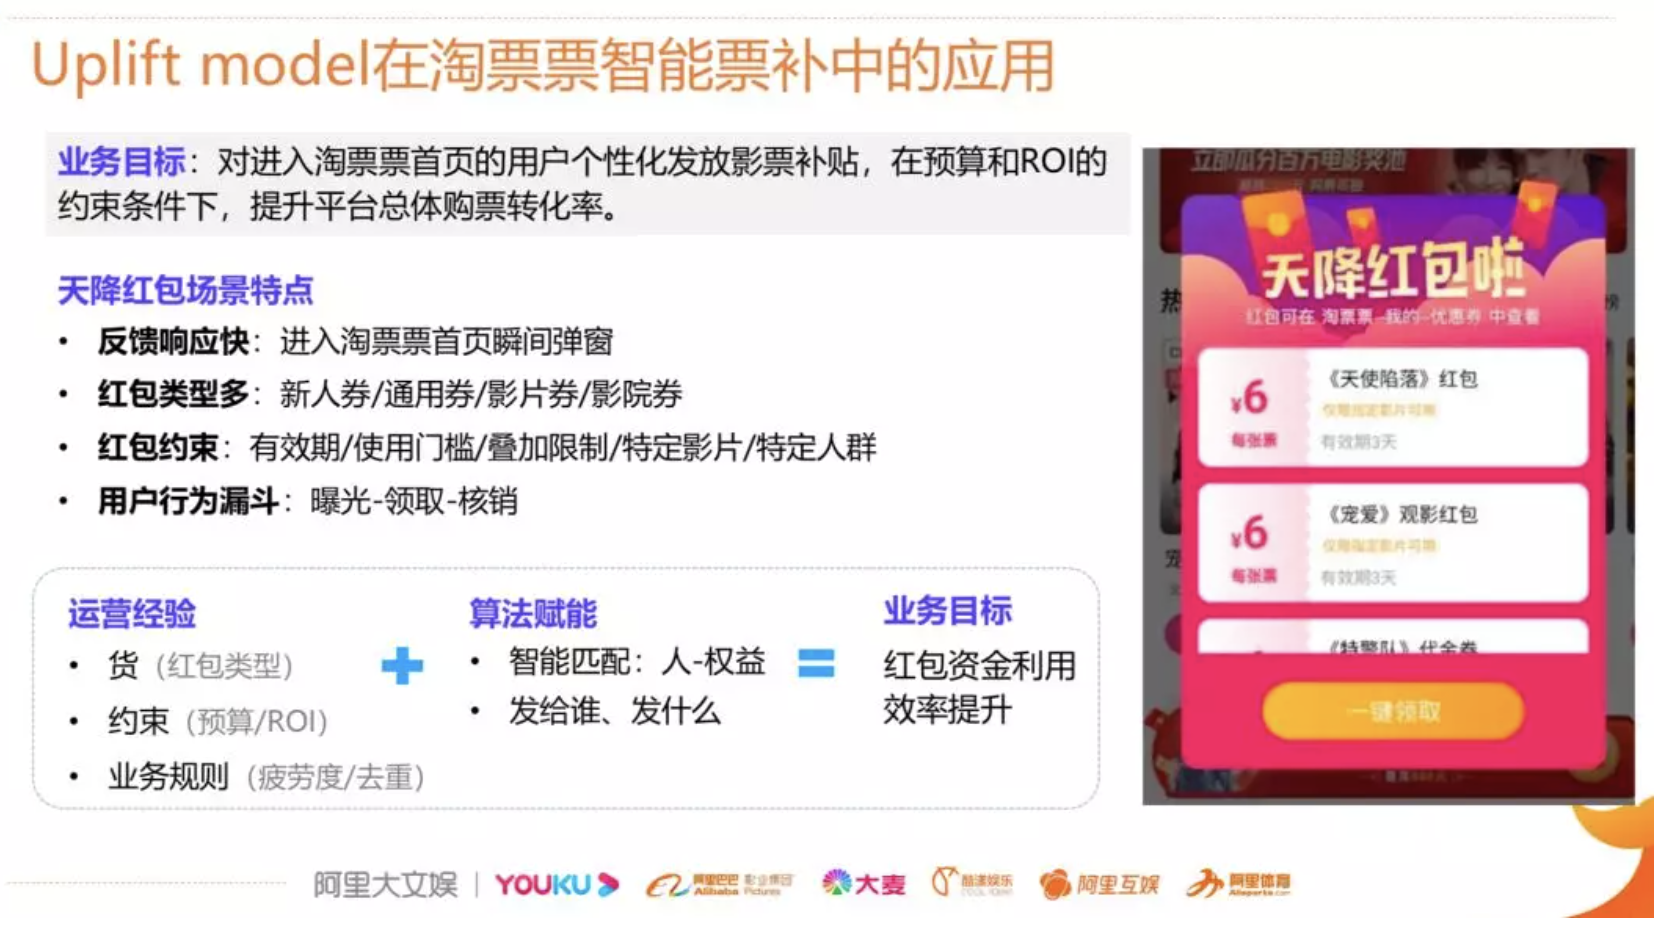
\includegraphics[width=1\textwidth]{fig/CasualInference-Uplift-Model-In-Ali.png}
\end{figure}

我们以平台通用券为例来说明问题是如何抽象和形式化的。在该场景下,每个用户最多只能发放一个红包,同时面额有固定几个分档,因此问题就精细化到如何对用户进行个性化的面额发放上,这可以通过经典的背包问题来抽象,如图所示,第一个公式是我们的目标,\textcolor{red}{最大化的是红包撬动效率,下面的约束条件一个是ROI约束,一个是预算约束}。目标函数公式中标红的部分是第$i$个用户在第$k$个红包下转化的uplift,$X_{ik}$是是否对用户$i$发放第$k$个红包,因此我们最终要决策的变量就是$X$矩阵。
\begin{figure}[H]
    \centering
    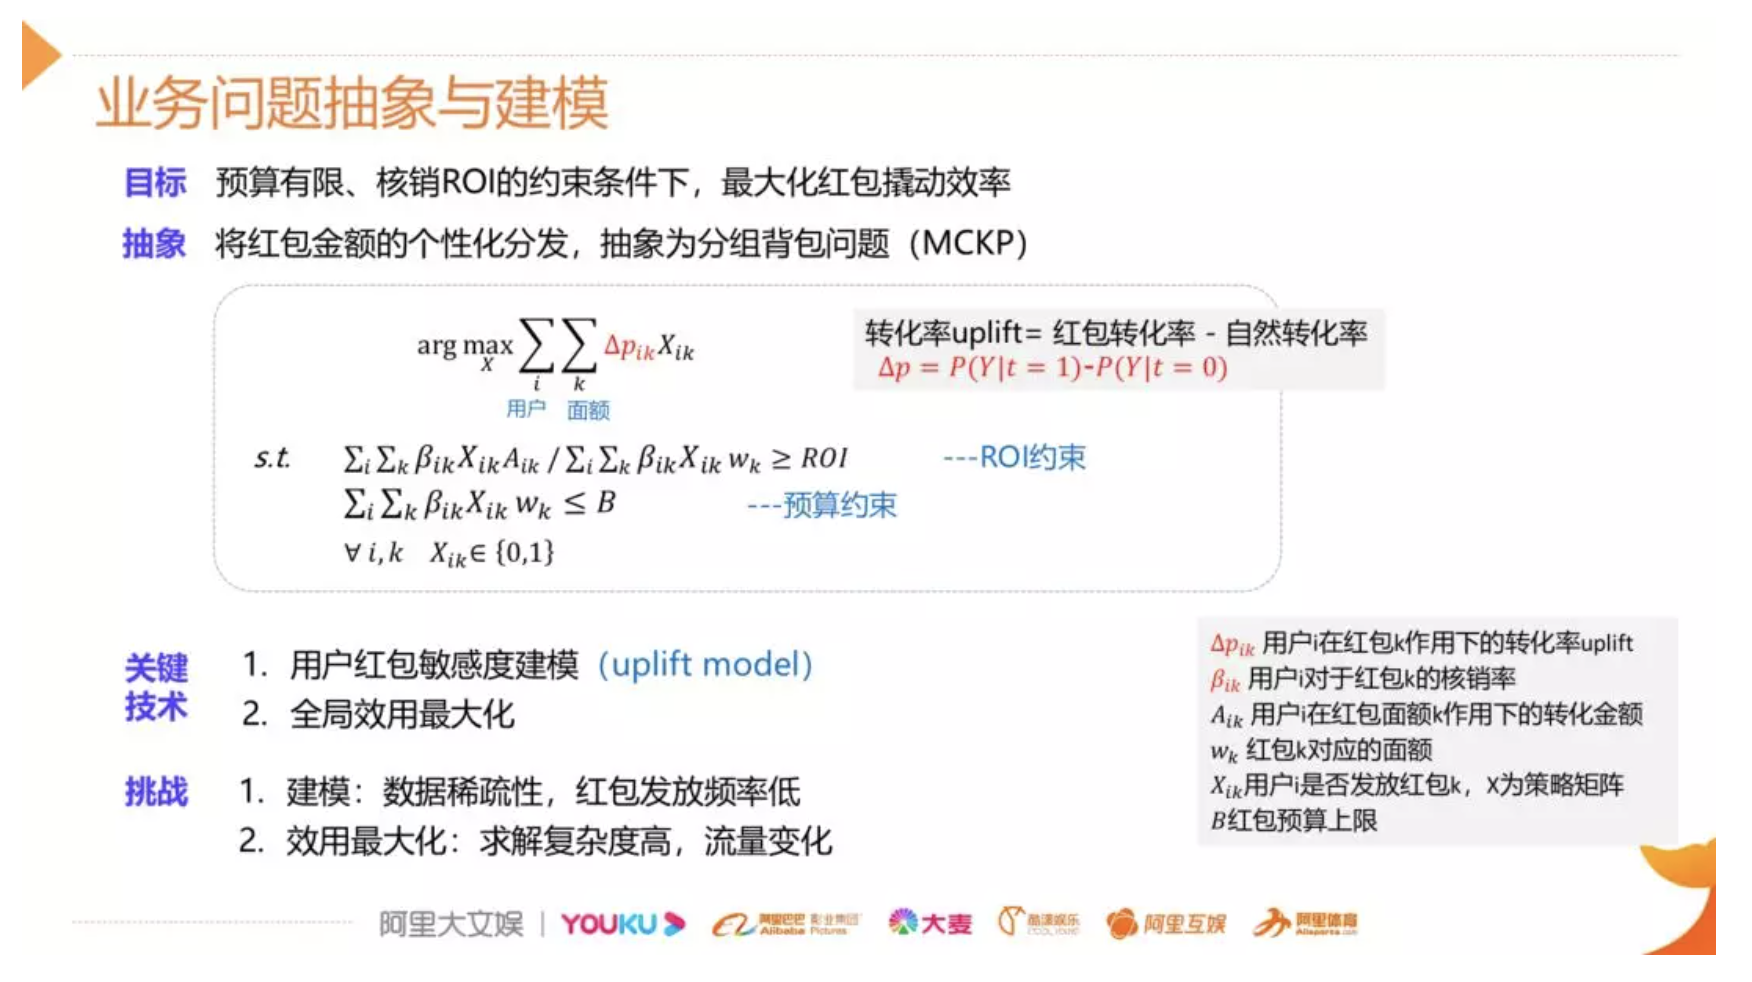
\includegraphics[width=1\textwidth]{fig/CasualInference-Uplift-Model-In-Ali2.png}
\end{figure}

\begin{align*}
\text{优化目标}: \qquad & \arg\max_x \sum_i\sum_k \Delta p_{ik}X_{ik}  \qquad(\text{其中,i代表用户维度,k代表券维度}) \\
\text{ROI 约束条件} \qquad & \sum_i\sum_k\beta_{ik}X_{ik}A_{ik} / \sum_i\sum_k\beta_{ik}X_{ik}w_k \ge ROI \\
\text{预算约束条件} \qquad & \sum_i\sum_k\beta_{ik}X_{ik}w_{k} \le B \\
& \forall i, k X_{ik} \in \{0, 1\}
\end{align*}

其中,转化率 uplift = 红包转化率 - 自然转化率,即$\Delta p = p(Y|t = 1) - P(Y|t = 0) $,即$\Delta p_{ik}$代表用户$i$在红包$k$下的转化率 uplift;

$\beta_{ik}$代表用户$i$对红包$k$的核销率;

$A_{ik}$代表用户$i$在红包面额$k$作用下的转化金额;

$w_{k}$代表红包$k$对应的面额;

$X_{ik}$代表是否对用户$i$发放红包$k$,$X$为策略矩阵;

$B$为红包预算上限;




该问题的求解中有两个关键点,一个是用户红包敏感度的建模,第二是在敏感度已知的情况下怎么进行全局效用最大化的求解。下面重点介绍uplift model模块。Uplift model的目标是预测每个用户在不同的红包金额下的转化率,从而构建出千人千面的敏感度曲线。
\begin{figure}[H]
    \centering
    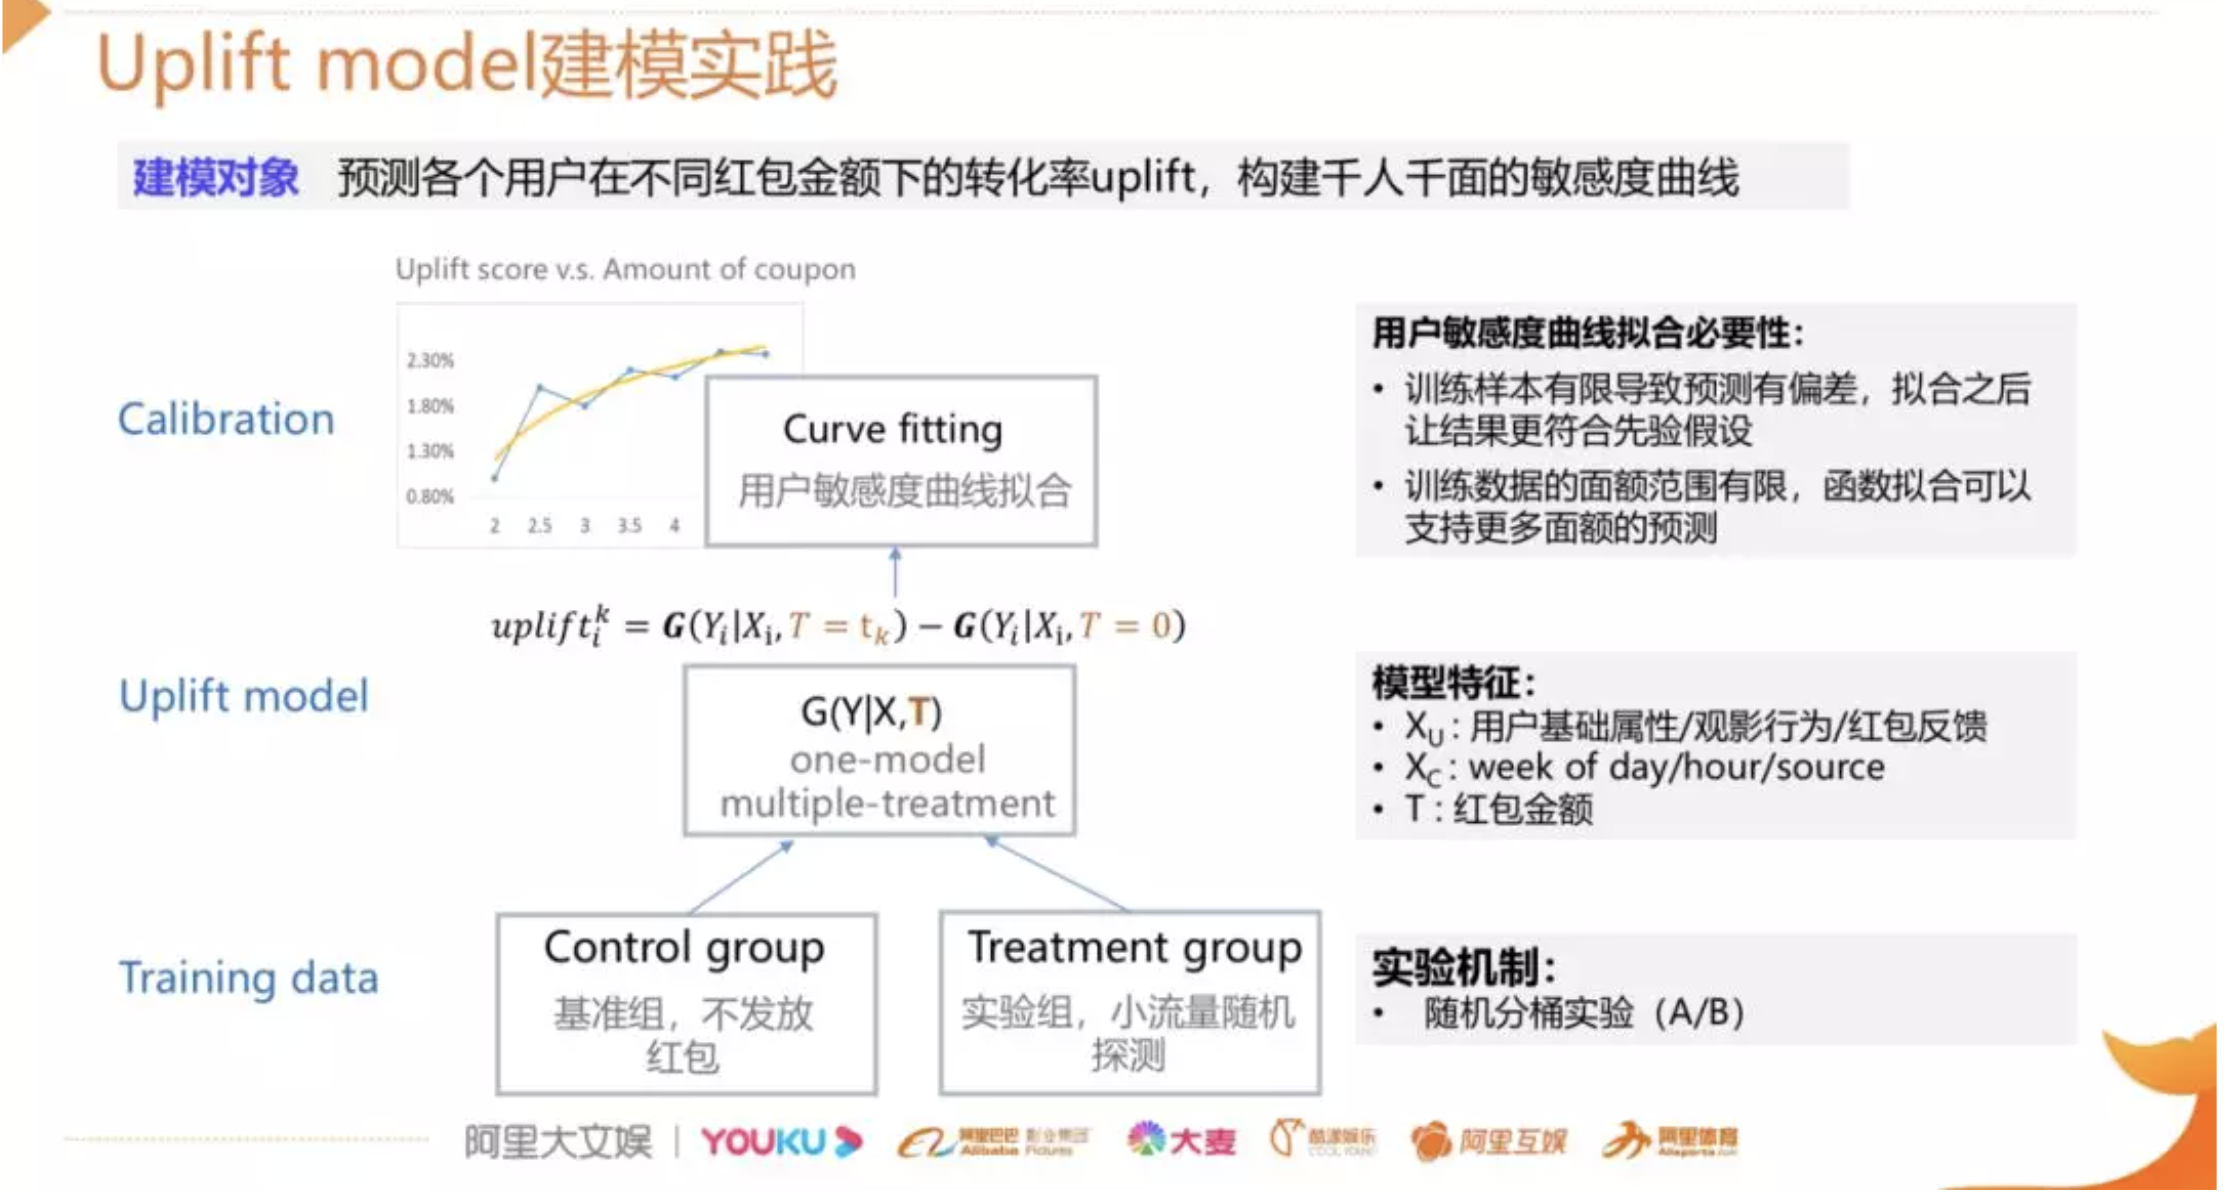
\includegraphics[width=1\textwidth]{fig/CasualInference-Uplift-Model-In-Ali3.png}
\end{figure}

我们将建模的任务拆分成三个步骤:

\textbf{ Step 1. 收集训练样本}

训练样本的收集和我们的实验是强相关的,我们采用的是随机化的分桶实验,它有两个好处,一是可以严谨公平地进行效果的评估,二是可以为uplift model的建模提供无偏的样本。建模中control组我们取的是随机化实验中的基准组,这部分用户是不进行红包发放的,而treatment组选用的是随机化实验中专为uplift model建模预留的一小部分随机探测的流量,之所以没有用有算法干预下的样本是因为用户的发放的面额与用户的特征是强相关的,并不满足CIA条件,因此这一部分样本虽然量较大,但是不能用于训练。

\textbf{ Step 2. 模型的构建和训练}

收集到样本之后可以进行建模,考虑到业务迭代的周期,我们使用的是前面介绍的One Model的差分响应模型,特征层面,除了user维度的基础属性,还有历史的观影行为,以及历史红包的反馈,同时也会引入线上实时的环境特征,最重要的是跟营销相关的特征T,目前T代表的是红包的金额。

\textbf{ Step 2. 面向业务层的模型校准和优化}

理论上到模型训练完成,就可以直接把模型放到线上去应用了,但是在离线调研时,我们发现一个问题,我们绘制的用户敏感度曲线和我们的预期不太一样,并不是严格的平滑递增的走势。我们分析有两个可能的原因:

一是与我们整体的样本规模比较有限有关,因为这种无偏样本目前大概只有几百万的量级;

二是由于用户行为的稀疏性,在这种场景下我们比较难收集到用户在不同面额下的历史数据,因此也会加剧这种不平滑性。

针对该问题,我们做了校准处理,把原始曲线做了一个函数的拟合,一方面可以让结果更加符合我们先验的假设,一方面经过这种函数化之后可以在后续支持更多面额的预测,但这种做法是否是最优的还值得进一步探讨。

\begin{figure}[H]
    \centering
    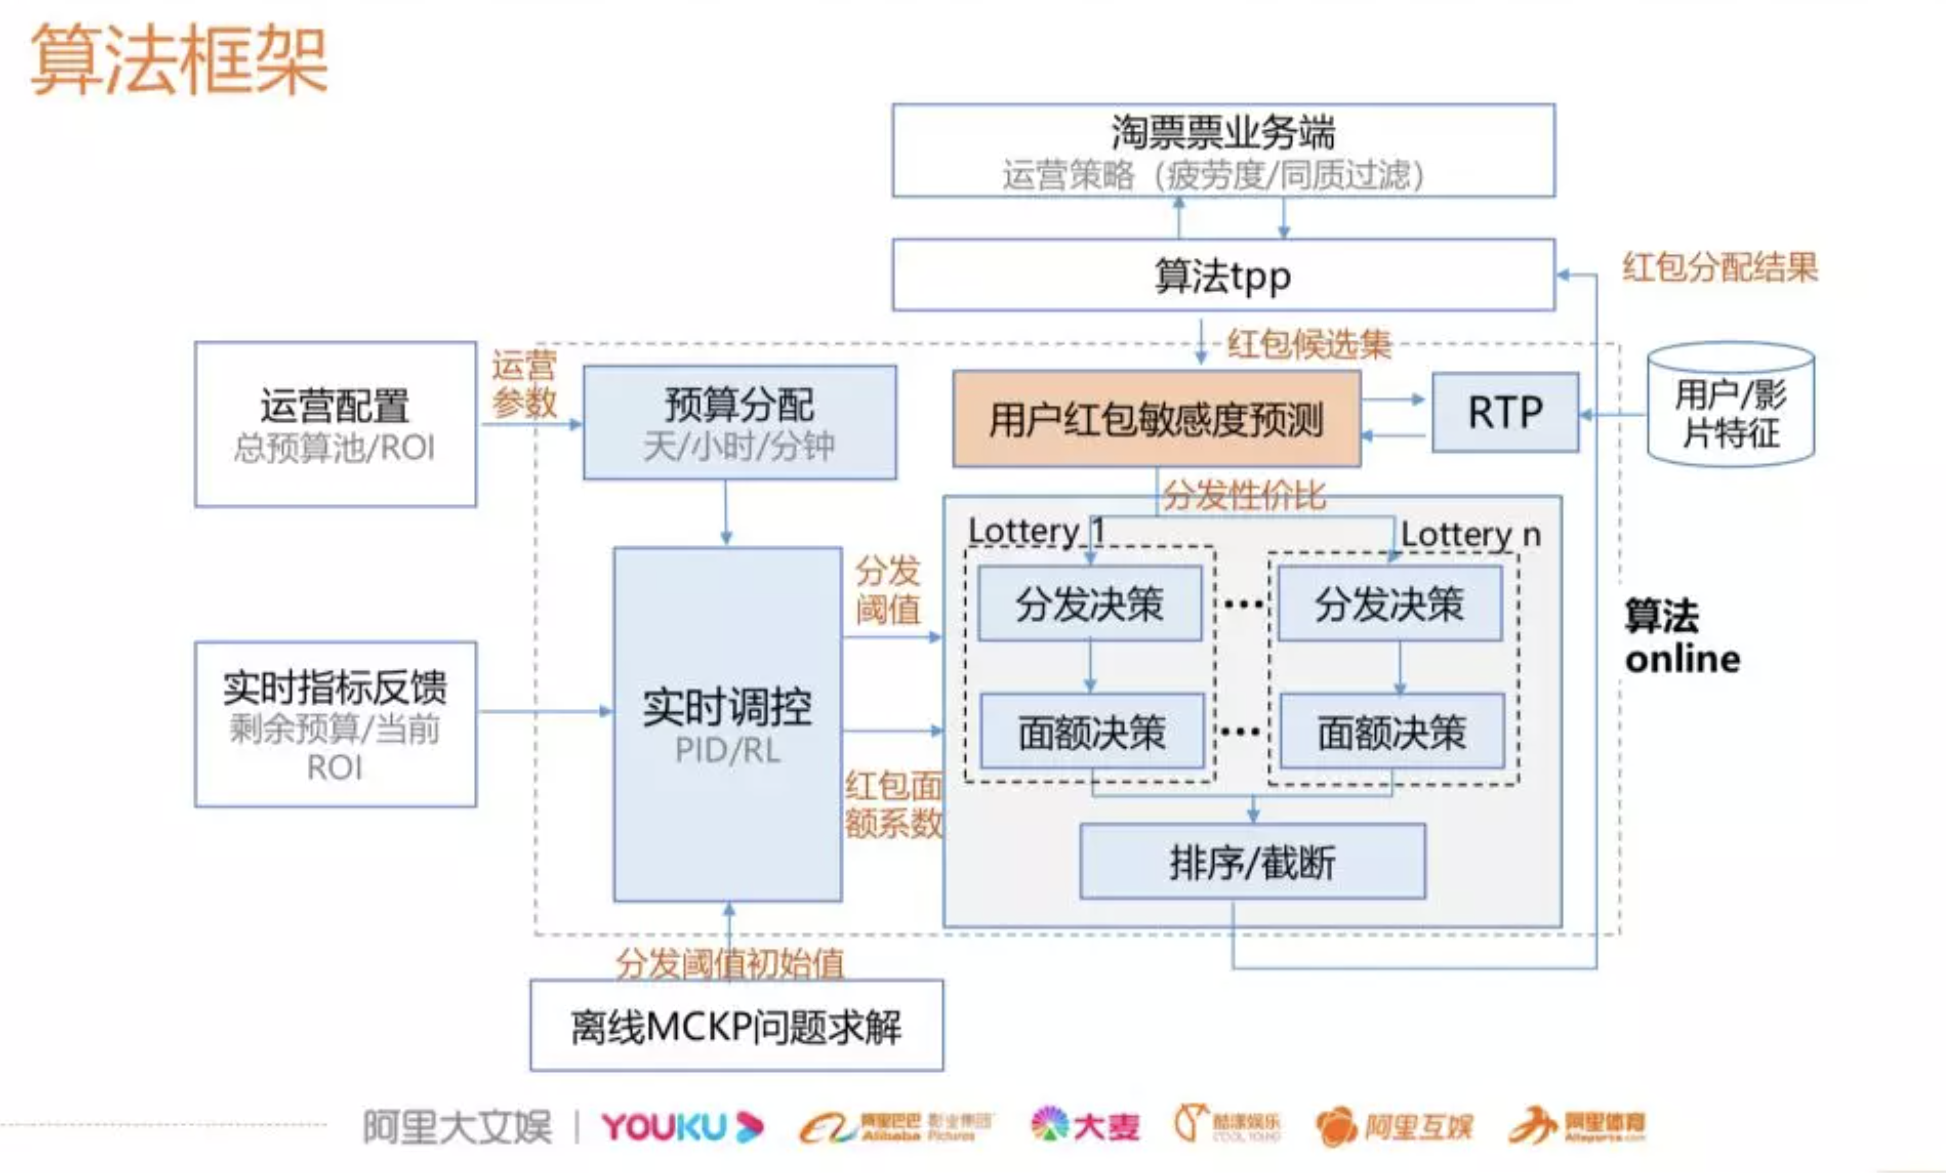
\includegraphics[width=1\textwidth]{fig/CasualInference-Uplift-Model-In-Ali4.png}
\end{figure}

模型在线上应用的框架图,如上图所示,黄色区域是基于uplift model的实时预测的模块,当一条用户的请求过来的时候,我们会实时去数据库中取用户的特征以及影片的特征,同时结合当前的环境特征预测用户在当前状态下真实的敏感度,基于这个敏感度可以进行后续分发的面额决策等。

\textbf{技术思考与后续规划}
之后智能营销的发展态势是营销手段会越来越复杂,玩法也会越来越多,比如之前我们发放的更多是平台的通用券,后面也会发一些和影片相关的影片券或者影院券,这意味treatment的维度是在不断增长的,除了红包的金额之外还需要考虑不同的红包类型,这会给算法带来两个方面的挑战,一是我们需要对问题的建模形式做一个升级,除了之前单一维度的建模之外,我们可能还要考虑多维度的建模,同时维度的剧增会对样本的量级要求越来越高,样本的稀疏性问题会更加严重,针对这个问题我们有两个可能的解法:

(1) 可以采用多任务学习的方式,联合其他场景一起建模缓解单场景样本的压力,同时也可以通过人为构造无偏样本的方式增加整体的样本量。当然除了技术侧,整个营销上面还有非常多很有意思的研究方向,比如之前更多考虑的是单个营销场景,但其实多个场景下怎么去建模和刻画他们之间的相互影响也是非常有意思的课题;

(2)我们之前uplift model建模更多考虑的是单次或者短期用户行为的增益,但实际上的营销往往是常态化或持续化的,用户的心智可能会不断发生变化,如何去建模长期的uplift也值得进一步去探讨。

%\printbibliography
\bibliography{../ref}
\bibliographystyle{IEEEtran}
\end{document}